\documentclass{sig-alternate}

\usepackage{amsmath}
\usepackage{graphicx}
\usepackage{subfigure}
\usepackage{color}
\usepackage{xspace}
\usepackage{url}
 \usepackage[utf8]{inputenc}

 % lorem
\newcommand{\lorem}               {\textcolor{green}{Lorem ipsum dolor sit amet, consectetur adipisicing elit, sed do eiusmod tempor incididunt ut labore et dolore magna aliqua. Ut enim ad minim veniam, quis nostrud exercitation ullamco laboris nisi ut aliquip ex ea commodo consequat. Duis aute irure dolor in reprehenderit in voluptate velit esse cillum dolore eu fugiat nulla pariatur. Excepteur sint occaecat cupidatat non proident, sunt in culpa qui officia deserunt mollit anim id est laborum.}}

% reviews
\newcommand{\thomas}[1]             {\textcolor{blue}{[Thomas] #1}}
\newcommand{\javier}[1]             {\textcolor{purple}{[Javier] #1}}
\newcommand{\keoma}[1]              {\textcolor{cyan}{[Keoma] #1}}
\newcommand{\remy}[1]               {\textcolor{yellow}{[Remy] #1}}
\newcommand{\jonathan}[1]           {\textcolor{pink}{[Jonathan] #1}}

% shortcuts
\newcommand{\name}                  {PEACH\xspace}
\newcommand{\smip}                  {SmartMesh~IP\xspace}

\graphicspath{{figures/}}

\begin{document}
\title{Feedbacks from a real-world low-power wireless sensor network deployment}

\numberofauthors{5}
\author{
  \alignauthor Brun-Laguna Keoma\\
    \affaddr{Inria, EVA team, Paris, France}\\
    \email{keoma.brun@inria.fr}
  \alignauthor Vilajosana Javier\\
    \affaddr{Universitat Oberta de Catalunya, Barcelona, Catalonia, Spain}\\
    \email{xvilajosana@uoc.edu}
  \alignauthor Léone Rémy \\
    \affaddr{Inria, EVA team, Paris, France}\\
    \email{remy.leone@inria.fr}
  \and
  \alignauthor Muñoz Jonathan\\
    \affaddr{Inria, EVA team, Paris, France}\\
    \affaddr{Gridbee, France}\\
    \email{jonathan.munoz@inria.fr}
  \alignauthor Watteyne Thomas \\
    \affaddr{Inria, EVA team, Paris, France}\\
    \email{thomas.watteyne@inria.fr}
}

\maketitle

\begin{abstract}
\lorem
\end{abstract}


%==============================================================================
\section{Introduction}
\label{sec:intro}

% the PEACH project

In April 2016, three research teams from different countries joined to start the deployment of a frost events prediction system~\cite{watteyne16peach}.
The goal of this project is to be able to precisely predict frost events and consequently reduce the impact of frost on peach production.
Low temperatures have a very harmful impact on peach production as in 2013, 85\% of the production in the Mendoza region (western Argentina) was lost because of frost.
Frost detection systems already exist but few actually able to propose prediction.

% the architecture

The deployed solution is composed of a low-power wireless network and a back-end system to retrieve and visualize the data.
The network is formed by \smip devices from the Linear Technology company and is in charge of measuring the orchard environment, gather the data into a gateway and pass it to the back-end system.
Both sensor values and network statistics are collected.
The back-end system stores and backups the data and provide both a visual interface and an API to access the data minutes after it was measured in Argentina.

% the deployment

The low-power wireless network is composed of 21 nodes uniformly distributed between the peach trees.
The covered area is an orchard with 204 trees on a 50*100m surface.
Each network mote is placed inside a water-tight box that is fixed on a 4m pole~\ref{fig:orchard}.
Because the project is on its first stage, we only measure air temperature from built-in sensors.
During the second stage, we will introduce additional sensors such as air temperature at different high, air relative humidity, soil moisture and soil temperature.

\begin{figure}
    \centering
    \includegraphics[width=\columnwidth]{orchard}
    \caption{The wireless motes deployed inside the orchard in Mendoza (Argentina)}
    \label{fig:orchard}
\end{figure}

% the technology

The \smip motes are based on the IEEE 802.15.4e standard that includes a channel hopping mechanism to reduce the impact of multipath fading.
Channel hopping exploit the frequency diversity to reduce the probability of interferences and improve link reliability.
This mechanism show good results in the Wireless Sensor Network (WSN) context~\cite{watteyne2010mitigating, watteyne2009reliability} and allows to achieve high reliability while saving energy.

% the data

Each mote produce a temperature value every 30 seconds and network statistics, called ``health-reports'', every 5~minutes.
In 3~months, we gathered more than 2M~temperature value, and more than 180K~network statistics.
The health reports produced by any mote contain information about the mote itself and also about its neighbors.
%65184 HR_DEVICE, 63245 HR_DISCOVERED and 50285 HR_NEIGHBORS


\lorem

% the goal of this paper

The goal of this paper is to present the first feedbacks we have from the 3-month-old project and the lessons we learned from deploying WSN in real environment.
\lorem

% paper organisation
This paper is organized as follow:
Section~\ref{sec:collected} gives an in-depth description of the data we collect.

\lorem

%==============================================================================
\section{Collected Data}
\label{sec:collected}

% health report description

Each device in the network produce both sensor data and network statistics.
Network statistics can be separated in \textbf{Events} and \textbf{Health Reports} messages.
The Events messages are non periodic information triggered for instance when a node join the network or when a link (layer 2) is created/deleted.
The Health Report (HR) message are sent periodically and provide counters and statistics to assess the overall network health.
There are three types of HR:
\begin{itemize}
  \item HR\_DEVICE give information about the mote itself
  \item HR\_NEIGHBORS give information about the mote active neighbors
  \item HR\_DISCOVERED give information about the mote potential neighbors
\end{itemize}
Each device sends one type of Health Report every 5~min making the complete set of Health Report generated every 15~min.

%------------------------------------------------------------------------------
\subsection{HR\_DEVICE}

\keoma{should we actually put all the technical details here ?}
An HR\_DEVICE message contains the following fields:
\begin{tabular}{l|p{6cm}}
    field name      & description\\
    \hline
    charge          & node charge in mC\\
    queueOcc        & mean and max queue occupancy.\\
    temperature     & built-in temperature sensor value in C\\
    batteryVoltage  & node battery voltage in mV\\
    numTxOk         & number of packets sent from NET to MAC\\
    numTxFail       & number of packets not sent due to congestion or failure to allocate a packet\\
    numRxOk         & number of packets received\\
    numRxLost       & number of packets lost (discarded by NET layer due to misc errors)\\
    numMacDropped   & number of packets dropped by MAC (due to retry count or age or no route)\\
    numTxBad        & transmit failure counter for bad link\\
    badLinkFrameId  & frame id of link with the worst performance over the last health report interval\\
    badLinkSlot     & slot of link with the worst performance over the last health report interval\\
    badLinkOffset   & offset of link with the worst performance over the last health report interval\\
\end{tabular}

% HR_DISCOVERED

\lorem

% HR_NEIGHBORS

\lorem

%==============================================================================
\section{RSSI}
\label{sec:rssi}

% RSSI expectations

The RSSI values can be retrieved from both active neighbors and discovered neighbors Health Reports, thus every 15~min for each pair of device.
Those RSSI values are average values over the 16 channels defined in the IEEE 802.15.4standard.
The peach orchard is located in a rural area that is not exposed to high traffic on the ISM band so we do not expect important external interferences.
Heavy machinery is used by farmers inside the orchards and could create internal interferences such as multipath fading.
Because the network exploits frequency diversity by using channel hopping techniques and that RSSI values are averaged over the all the channels, we should observe a relatively constant values on short period of time.

%------------------------------------------------------------------------------
\subsection{Time pattern}

By looking at the data, we can observe a clear day-periodic pattern on some of the motes.
Figure~\ref{fig:periodic_rssi} presents the average RSSI value of node 60-03-82 as received by node 60-08-d5 over a week.
The RSSI value range from -86 to -76~dBm and correspond with midday and midnight hours respectively.
That is, average RSSI can be 8~dBm better during the night than during the day.

\begin{figure}
    \centering
    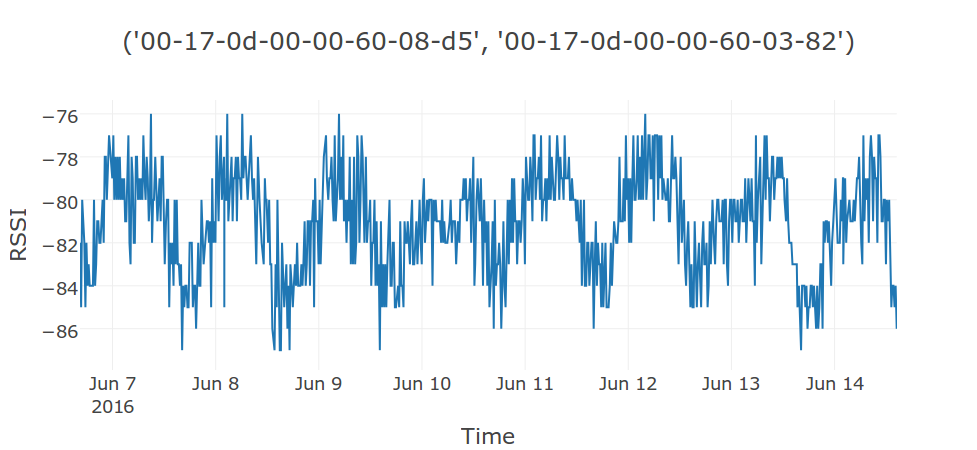
\includegraphics[width=\columnwidth]{periodic_rssi}
    \caption{The average RSSI value of node 60-03-82 as received by mote 60-08-d5 over a week. A clear day periodicity can be observed.}
    \label{fig:periodic_rssi}
\end{figure}

Although we are not able to prove this assumption with our current data, one possible explanation can be the impact of temperature and humidity on RSSI~\cite{luomala15effects}.

%------------------------------------------------------------------------------
\subsection{Variation}

As said previously, average RSSI should remain relatively constant due to channel hopping.
Figure~\ref{fig:rssi_variation} shows that the difference between two consecutive average RSSI values does not go above 6dBm and has a standard deviation of 1.56 dBm.
This variation is low considering that we have 15~min sampling period.

\begin{figure}
    \centering
    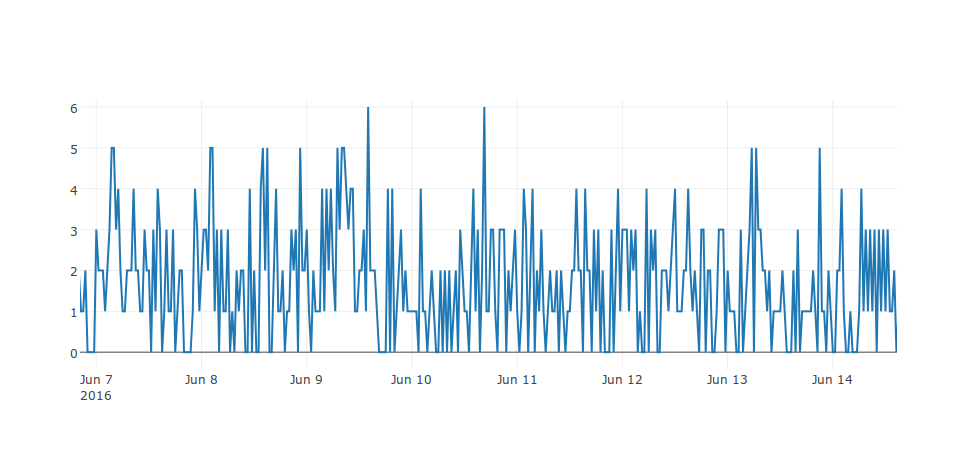
\includegraphics[width=\columnwidth]{rssi_variation}
    \caption{The variation of average RSSI value of node 60-03-82 as received by mote 60-08-d5 over a week. Variation are small considering the 15~min sampling rate.}
    \label{fig:rssi_variation}
\end{figure}

%------------------------------------------------------------------------------
\subsection{RSSI and Distance}

\lorem

\begin{figure}
    \centering
    
\includegraphics[width=\columnwidth]{fake}
    \caption{The famous Pister-Hack model here}
    \label{fig:rssi_dist}
\end{figure}

%==============================================================================
\section{PDR}
\label{sec:pdr}

% intro

% PDR periodicity/patterns
\lorem

\begin{figure}
    \centering
    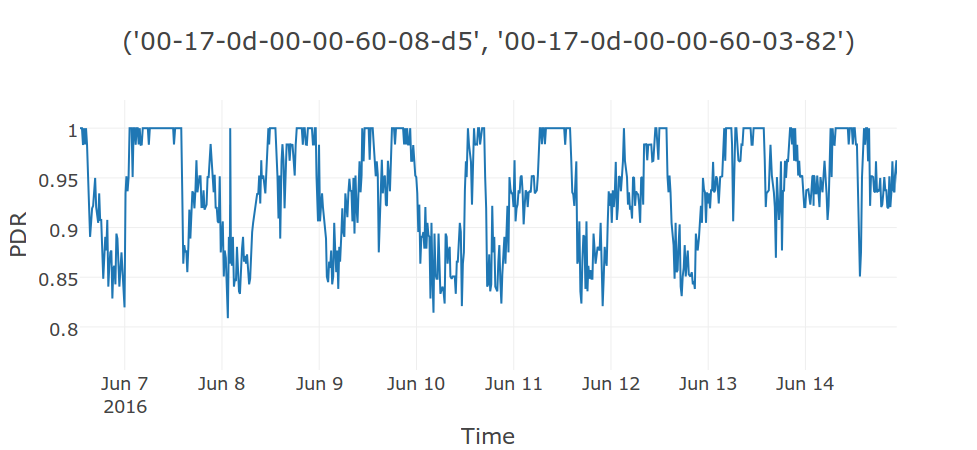
\includegraphics[width=\columnwidth]{periodic_pdr}
    \caption{The PDR when node 60-08-d5 sends data to 60-03-82 over a week.}
    \label{fig:periodic_pdr}
\end{figure}

% PDR and distance

\lorem

\begin{figure}
    \centering
    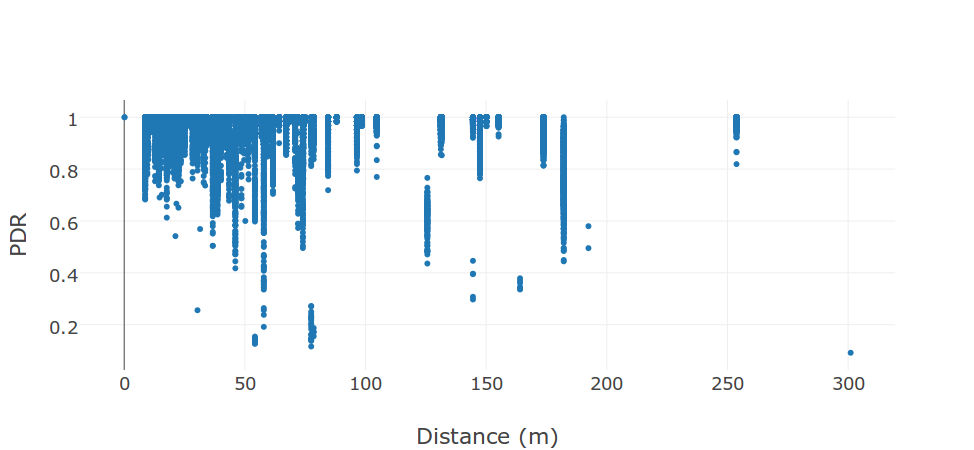
\includegraphics[width=\columnwidth]{pdr_dist}
    \caption{The relation between PDR and distance. No pattern or trend are visually identifiable.}
    \label{fig:pdr_dist}
\end{figure}

%==============================================================================
\section{Topology}
\label{sec:topology}

% topology expectations

\lorem

% what we found

\lorem

\begin{figure}
    \centering
    
\includegraphics[width=\columnwidth]{fake}
    \caption{Network churn here}
    \label{fig:net_churn}
\end{figure}

% network load distribution

\lorem

\begin{figure}
    \centering
    
\includegraphics[width=\columnwidth]{fake}
    \caption{Load distribution here}
    \label{fig:net_flows}
\end{figure}

%==============================================================================
\section{Reliability}
\label{sec:reliability}

% reliability expectation

\lorem

\begin{figure}
    \centering
    
\includegraphics[width=\columnwidth]{fake}
    \caption{The RSSI value of node 0f-66 as received by mote 03-82 over a week.}
    \label{fig:reliability}
\end{figure}

%==============================================================================
\section{Technology Feedbacks}
\label{sec:technology}
\keoma{is this section relevant ?}
% intro (why is this section relevant)

\lorem

% SOL

\lorem

% database

\lorem

% grafana

\lorem

%==============================================================================
\section{Conclusion}
\label{sec:conclusion}

% conclusion

\lorem

%==============================================================================

\bibliographystyle{abbrv}
\bibliography{16chants}

\end{document}

%
